%!TEX TS-program = pdflatex
\documentclass[a4paper,12pt,twoside]{article}

\usepackage{mathptmx}
\usepackage{parskip}
\usepackage[top=1.5in,left=1in,right=1in,bottom=1in]{geometry}
%\setlength{\parindent}{0pt}
%\setlength{\parskip}{\the\baselineskip}
\pagestyle{empty} 

\makeatletter
\renewcommand\@makefntext[1]{%
  \parindent 1em\noindent
  \hbox{\@makefnmark}#1}
\renewcommand\large{\@setfontsize\large{14pt}{18}} % For standardizing with the Word template: normally \large is 14.4pt
\makeatother
\usepackage{titlesec}
\titleformat{\subsection}{\normalfont\normalsize}{\thesubsection.}{1ex}{}
\titleformat{\subsubsection}{\normalfont\normalsize}{\thesubsubsection.}{1ex}{}
\titleformat{\section}{\normalfont\normalsize\bfseries}{\thesection.}{1ex}{}
% \titlespacing*{\section}{0pt}{*0}{0pt}
% \titlespacing*{\subsection}{0pt}{\the\baselineskip}{0pt}

\usepackage{natbib} 
\bibpunct{(}{)}{;}{a}{,}{,}


\setlength{\bibsep}{0pt} \relax
\setcitestyle{notesep={: },yysep={, }} \relax

\usepackage{linguex,url}
\def\refdash{} % To suppress the dash in (2-a) etc. Defining both as different versions of linguex had different names for this command.
\def\firstrefdash{}


\usepackage{titleps}
\usepackage{lipsum}
\newpagestyle{mystyle}{
\sethead[\thepage][\Author][]{}{\Title}{\thepage}
}
\pagestyle{mystyle}
\author{Hofmann \and de Marneffe  \and Tonhauser}
\title{Projection variability of clausal complements across different operators}
\makeatletter
\newcommand\Author{Hofmann, de Marneffe, and Tonhauser}
\let\Title\@title
\makeatother
%header with author and title

\pagenumbering{gobble} 
%suppresses page numbering in header


%!TEX root = projection-operators-SuB.tex

%% extra

% misc formatting
	\usepackage{booktabs}
	\usepackage[export]{adjustbox}

%% bibliography
	\newcommand{\posscite}[1]{\citeauthor{#1}'s (\citeyear{#1})}
	% \renewcommand*{\refname}{\normalsize\textbf{References}\\ \vspace{-.5\baselineskip}}
	% \newcommand{\citepos}[1]{\citeauthor{#1}'s \citeyear{\#1}}
	% \newcommand{\citeposs}[1]{\citeauthor{#1}'s}
	% \newcommand{\citetpos}[1]{\citeauthor{#1}'s (\citeyear{\#1})}

% drawing
	% \usepackage{tikz}
	\usepackage{graphicx}
	\usepackage{xcolor}

% % symbols 
% 	\usepackage{pifont}% http://ctan.org/pkg/pifont
% 	\newcommand{\cmark}{\ding{51}}%
% 	\newcommand{\xmark}{\ding{55}}%




\begin{document}
%%\maketitle
\setlength{\Extopsep}{0pt}
\thispagestyle{empty}

{\large \textbf{Projection variability of clausal complements across different operators}}\footnote{We would like to thank\ldots }\\
Lisa HOFMANN --- \textit{University of Stuttgart}\\
Marie-Catherine DE MARNEFFE --- \textit{UC Louvain}\\
Judith TONHAUSER --- \textit{University of Stuttgart}\\

\textbf{Abstract.}
	We present experimental evidence that the projection of clausal complements \textbf{(i)} varies among entailment-canceling operators, \textbf{(ii)} that the effect of operator varies between clause-embedding predicates, and \textbf{(iii)} we extend the result from \citet{degen_are_2022}, that projection ratings in polar questions are gradient in ways that cannot be predicted by categorical lexical classes, to contexts with negation, the epistemic possibility modal \textit{perhaps}, and conditional antecedents.
	%
	The observed variability is not captured by existing theoretical accounts of projection
	(e.g., \citealt{heim_projection_1983,van_der_sandt_presupposition_1992,abrusan_predicting_2011,schlenker_triggering_2021}).
	%
	Our results suggest that an analysis must consider interactions between predicates and operators and raise important questions for future research on projection.	

\textbf{Keywords:} projection, commitment, discourse interpretation.


\section{Introduction}
	Language users may infer that a speaker who uses a clause-embedding predicate, as in \ref{ex:family}, is committed to the content of the complement (CC, here: \emph{Julian dances salsa,}) even when it occurs under an entailment-canceling operator, like negation \ref{ex:neg}, polar questions \ref{ex:q}, epistemic possibility modals \ref{ex:mod}, or conditional antecedents \ref{ex:cond}, in which case we say that it \textit{projects} (e.g., \citealt{frege_uber_1892,strawson_referring_1950,kiparsky_fact_1970,karttunen_conventional_1979}).

	\ex. \label{ex:family}
		\a. \label{ex:neg}
			{\bf Negation:} \hfill
			\emph{\lq Cole didn't discover that Julian dances salsa.\rq}
		\b. \label{ex:q}
			{\bf Polar Question:} \hfill
			\emph{\lq Did Cole discover that Julian dances salsa?\rq}
		\c. \label{ex:mod}
			{\bf Modal:} \hfill
			\emph{\lq Perhaps Cole discovered that Julian dances salsa.\rq}
		\d. \label{ex:cond}
			{\bf Conditional:} \hfill
			\emph{\lq If Cole discovered that Julian dances salsa, Logan will be joyful.\rq}
		\z.
	\z.
	
	We investigate whether the projection of embedded propositional content from under entailment-cancelling operators differs by operator and whether by-operator differences vary between embedding predicates.
	%
	Textbook diagnostics for projection often assume that if a content projects across one of the operators in \Last, it uniformly projects across the others (e.g., \citealt{chierchia_meaning_1990}). Accordingly, current research examines projection variability between these operators only rarely and with conflicting findings.
	
	\citet{karttunen_observations_1971} proposed a distinction between English factive predicates (e.g., \textit{be annoyed, regret, reveal, know}), where the CC projects across all four operators, and semi-factives (e.g., \textit{discover, realize, see, notice, find out}) where it always projects from under negation, but not always from under polar questions, modals, or conditionals. 

	\citet{smith_relationship_2014} investigated by-operator variation, comparing negation and conditionals, for various types of projective content. They found that the expressive content of epithets (e.g. \textit{idiot}) and the CC of \textit{know} was more projective under negation than conditionals, whereas appositive relative clauses and the preparatory content of \textit{win} showed the opposite pattern, and the existential presupposition of clefts showed no difference. However, their task involved asking participants how surprised they would be to learn the content under investigation after observing the utterance. Since other factors besides speaker commitment modulate discourse (un)expectedness \citep[see e.g.][]{zimmermann_grammatical_2011,tonnis_german_2021}, it is unclear that they (only) measured projection. 

	\posscite{sieker_projective_2022} study on German clause-embedding predicates compared the projection of purported factives (\textit{wissen} `know', \textit{bereuen} `regret', \textit{enthüllen} `reveal') and semi-factives (\textit{bemerken} `notice', \textit{entdecken} `discover', \textit{herausfinden} `find out') across the four contexts in \Last. They replicated Smith and Hall's result that the CC of \textit{know} projects more from under negation than conditionals for German \textit{wissen} (`know'). However, this finding was part of an overall pattern of higher projection ratings with negation than other operators.
	%
	Importantly, their analysis did not explore the impact of operators on each predicate individually. Instead, it grouped ratings for the four purported factive and semi-factive predicates, respectively. Based on this analysis, they found no interaction of operator with predicate type, and thus no evidence for the distinction of factives vs. semi-factives.

	Studies in \citet{djarv_cognitive_2018}, \citet{tonhauser_how_2018}, and \citet{degen_are_2022} observed by-predicate variation in polar questions, where Karttunen's classification predicts more projection for factives than semi-factives.
	%
	\citet{djarv_cognitive_2018}, assessing acceptability of affirming the main clause while denying the CC, did find higher ratings for \emph{be happy} and \emph{appreciate} (assumed to be factive) and \emph{be aware} than \emph{realize} (assumed to be semi-factive). But here, it is also not obvious how exactly this task relates to projection.\footnote{Say why}
	
	\citet{tonhauser_how_2018} and \citet{degen_are_2022} measured speaker commitments towards a broad range of projective contents more directly, by collecting judgments of how certain participants take a speaker to be of the contents under investigation.
	%
	The observed differences between CCs of various clause-embedding predicates do not align with theoretically assumed lexical classes. While \citet{degen_are_2022} demonstrate this for the distinction between purported factive and non-factive predicates, the results did not match the expectations from Karttunen's factive vs. semi-factive classification either.
	%
	\citet{tonhauser_how_2018} found, e.g., that the CC of semi-factive \emph{realize} was as projective as that of factive \emph{be annoyed} and more than that of semi-factive \emph{discover}. \citet{degen_are_2022} observed that the CC of factive \textit{reveal} was less projective than that of semi-factive \textit{discover}, which, in turn, was less projective than that of factive \textit{know}. These findings suggest that examining projection ratings for various predicates individually, rather than pre-grouping them based on theoretical assumptions, can provide more nuanced insights into by-predicate projection variation.

	While \citet{smith_relationship_2014} found by-predicate variation in the effect of the operator on projection, \citet{sieker_projective_2022} did not.
	%
	These divergent results raise the question if they are due to cross-linguistic variation, task differences, or artifacts of the analysis. To address this, we conducted a series of experiments designed to assess projection across the four entailment-canceling operators in \ref{ex:family}. We used the same projection measure as \citet{sieker_projective_2022} (the `certain that' diagnostic; see e.g., \citealp{tonhauser_how_2018,djarv_prosodic_2017,mahler_social_2020}) and applied it to the CC of 20 English clause-embedding predicates, including factive and semi-factive predicates, and 15 non-factive predicates, given recent findings that their complements may also project, albeit to varying degrees (\citealt{degen_are_2022}).


\section{Assessing projection across entailment-canceling operators}

	To assess the effect of entailment-cancelling operators and clause-embedding predicates on the projection of the embedded content, we collected projectivity judgments for contents embedded under 20 clause-embedding predicates in four sets of experiments. The predicates were embedded under negation in Experiments~1, under polar questions (Exps.~2), under the epistemic possibility modal {\em perhaps} (Exps.~3), and in conditional antecedents (Exps.~4). Each set of experiments contained three experiments differing in an at-issueness measure used in a separate block. We focus on the projection ratings here.

		Projection was measured across all 12 experiments with the `certain that' diagnostic, which has been used to measure projection with both polar interrogative and declarative sentences (see, e.g., \citealt{tonhauser_prosodic_2016,djarv_prosodic_2017,stevens_rational_2017,lorson_influence_2018,tonhauser_how_2018,mahler_does_2019,mahler_social_2020,de_marneffe_commitmentbank_2019}).\footnote{For other diagnostics of projection see, e.g.\ \citealt{smith_projection_2011,xue_correlation_2011}, and \citealt{tonhauser_toward_2013}; and discussion in \citealt{tonhauser_how_2018}.} Participants were presented with utterances like those in \Next and judged whether the speaker (who was named) was certain of the CC (e.g.: Is Christopher certain that Julian dances salsa?).

		\ex. \label{ex:certain-that}
			\a. Christopher: \emph{\lq Cole didn't discover that Julian dances salsa.\rq}
			\b. Christopher: \emph{\lq Did Cole discover that Julian dances salsa?\rq}
			\c. Christopher: \emph{\lq Perhaps Cole discovered that Julian dances salsa.\rq}
			\d. Christopher: \emph{\lq If Cole discovered that Julian dances salsa, Logan will be joyful.\rq}
			\z.
			Projection question: Is Christopher certain that Julian dances salsa?
		\z.

		Following \citet{tonhauser_prosodic_2016,djarv_prosodic_2017,tonhauser_how_2018,lorson_influence_2018,mahler_does_2019}, we took a `yes' response to indicate that participants interpret the utterance in a way that the presented speaker (e.g., Christopher in \Last) is committed to the embedded content, which reflects projection. A `no' response was taken to indicate that the content does not project.
		%
		Based on Karttunen's generalization, we would expect the CC of semi-factive predicates to receive high projection ratings under negation and lower ratings under the other operators, while the CC of factive predicates would consistently receive relatively high projection ratings throughout.


	\subsection{Experimental method}

		\subsubsection{Participants}
			In each of the 12 experiments, 250-300 inhabitants of the USA participated via Prolific or Amazon's MT platform. 
			%
			We analyze the data from $2,682$ self-reported native speakers of American English, after excluding participants who failed one of the following two attention-checks: their mean rating on six control items is more than 2 sd different from the group mean, or they always roughly selected the same point on the scale for target stimuli (identified by low variance, and then manually inspecting their response patterns).

		\subsubsection{Materials and procedure }
			We tested 20 clause-embedding predicates \Next which have shown projection variability in question contexts (\citealt{degen_are_2022}). They comprise three purported factive predicates \Next[a], two purported semi-factives \Next[b], nine that have been characterized as optionally factive in \citealt{kiparsky_fact_1970} \Next[c], and six non-factives which include two veridical predicates \Next[d], and four non-veridical ones \Next[e].

			\ex. 20 clause-embedding predicates \hfill \citealt{degen_are_2022}
				\a. canonically factive:
					\hfill \emph{be annoyed, know, reveal}
				\b. semi-factive:
					\hfill \emph{discover, see}
				\b. optionally factive: \newline
					\phantom.\hfill \emph{acknowledge admit, announce, confess, confirm, establish, hear, inform, prove}
				\b. Non-factive veridical:
					\hfill \emph{be right, demonstrate}
				\b. Non-veridical:
					\hfill \emph{pretend, say, suggest, think}
				\z.
			\z.

			Each participant saw all 20 predicates, randomly paired with a unique embedded clause from a set of 20 contents, and a subject from a set of 20 proper names. The predicates associated with projective content were embedded under (i) negation, (ii) polar questions, (iii) the epistemic possibility modal \textit{perhaps}, and (iv) in conditional antecedents in the four different sets of experiments.

			On each trial, participants read an utterance and the corresponding projection question. They gave their response on a slider marked `no' (coded as 0) at one end and and `yes' (coded as 1) on the other. This is illustrated in Figure~\ref{fig:trial}. Following, e.g., \citet{tonhauser_how_2018}, we take high ratings of speaker certainty to reflect speaker greater speaker commitment towards the CC.

			\begin{figure}[ht]
				\centering
				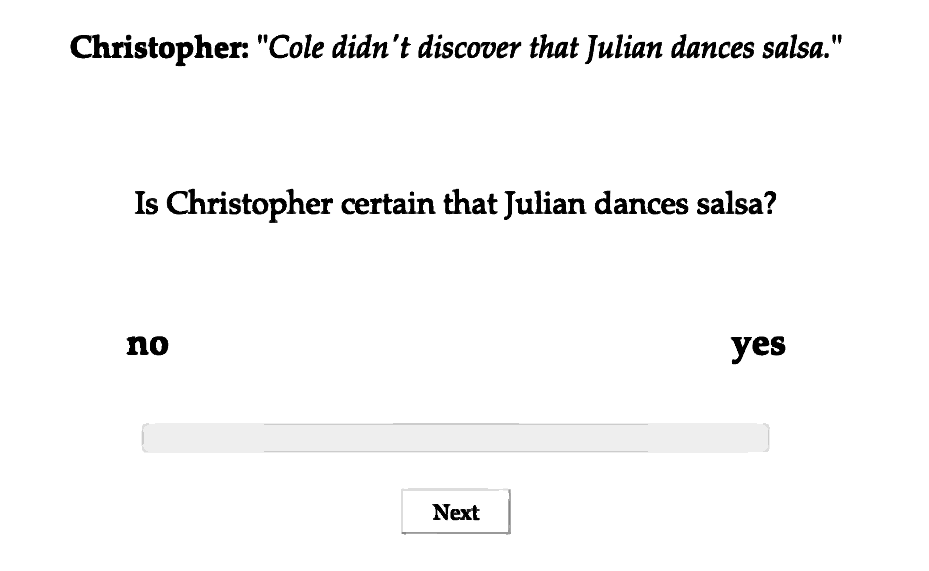
\includegraphics[width = .7\linewidth]{task-1n-proj.eps}
				\caption{A sample trial in Exp.~1. In the corresponding trials in Exps.~2-4, participants were presented with an utterance involving a different entailment-cancelling operator.}
				\label{fig:trial}
			\end{figure}

			Each experiment also included six control stimuli, which were main clauses with appositive relative clauses, which were also presented as utterances made by a named speaker. Here, the main clause content was targeted by the projection question. In the experiments with polar questions, the controls were expected to receive low certainty ratings, whereas in the experiments with declaratives, they were expected to receive high ratings.

			Participants were told to imagine that they are at a party and that, on walking into the kitchen, they overhear somebody say something to somebody else. Each participant saw a random set of 26 stimuli: each set contained one target utterance for each of the 20 contents (each paired with a unique clause-embedding predicates) and the same 6 (experiment-specific) control stimuli. Each participant saw their set of 26 stimuli twice, once in the projection block and once in the at-issueness block. Block order and within-block trial order was randomized. After completing the experiment, participants filled out a short optional demographic survey.

	\subsection{Results and discussion}
		Our data reveals three key results: \textbf{(i)} There is projection variability by operator; \textbf{(ii)} There is by-predicate variation in the effect of operator on projection; and \textbf{(iii)} We find further support (from entailment-cancelling operators beyond polar questions) for \posscite{degen_are_2022} result that by-predicate projection variation is gradient in a way that cannot be predicted by categorical lexical classes.
		
		\subsubsection{By-operator variation}
			When aggregating across predicates, we found an effect of \texttt{operator}. The distribution of projection ratings, as well as means and $95\%$ bootstrapped confidence intervals by operator are shown in Figure~\ref{fig:op-ratings}.

			\begin{figure}[ht]
				\centering
				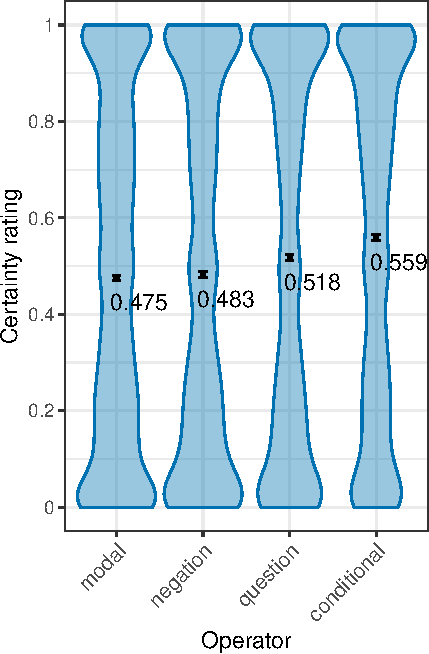
\includegraphics[scale = .8]{operator-graph-1}
				\caption{Certainty ratings by operator with means and $95\%$ bootstrapped confidence intervals.}
				\label{fig:op-ratings}
			\end{figure}

			Mean projection ratings were higher for CCs in question-embeddings than under negation and modals, but lower than in conditional antecedents. These generalizations are supported by Model \#1 reported in Table~\ref{t:op-model}.

			\begin{table}[ht]
					\centering
					\hspace{-1.3em}
					\begin{tabular}{llrrrr}
						Model & & Estimate & Std. Error & t-value\\
						\midrule
						\#1 & Intercept: \emph{question} & 0.51 & 0.01 & 44.78 & ***\\
						& operator: conditional & 0.05 & 0.01 & 5.30 & ***\\
						& operator: modal & -0.04 & 0.01 & -4.45 & ***\\
						& operator: negation & -0.03 & 0.01 & -4.67 & ***\\
						\bottomrule
					\end{tabular}
				
					\caption{Excerpt from the model output of a linear mixed effects model with fixed effects of operator; random effects: participant and item intercepts, fitted with \texttt{lme4, lmertest} in \texttt{R}.\label{t:op-model}}
				\end{table}

			Like \citet{sieker_projective_2022}, we observe a small main effect of entailment-cancelling operator on projection. However, our result, that the CC of clause-embedding predicates projects most from conditional antecedents and least from under negation and modals, differs from their finding that the CC of the German predicates they tested projects more from under negation than the other operators. Further, the projection ratings they report are overall quite a bit higher than the ones reported here (their overall mean is at around $0.855$, while ours is at around $0.501$).
			%
			We can understand these differences based on an effect of \texttt{predicate}, established in the upcoming subsections, and a different set of predicates tested in the two studies. While Sieker \& Solstad tested only predicates that are characterized as factive or semi-factive in the literature, yielding relatively high projection ratings, we also included ones that are usually characterized as non-factive, lowering the overall mean projection ratings. The difference in the direction of the effect of the operator between the two studies can also be tied to a different set of predicates tested, because the effect of operator on projection differs by predicate.

		\subsubsection{Gradient by-predicate variation}

			Taking into account the effect of \texttt{predicate} on projection, we find gradient projection variation, like \citet{tonhauser_how_2018} and \citet{degen_are_2022}.
			%
			This is illustrated in Figure~\ref{fig:op-pred-ratings}, which shows mean projection ratings for the 20 predicates grouped by embedding operator. Here, predicates on the x-axis are ordered by their mean rating across all operators (\emph{be annoyed} has the highest overall mean).

			\begin{figure}[ht]
				\centering
				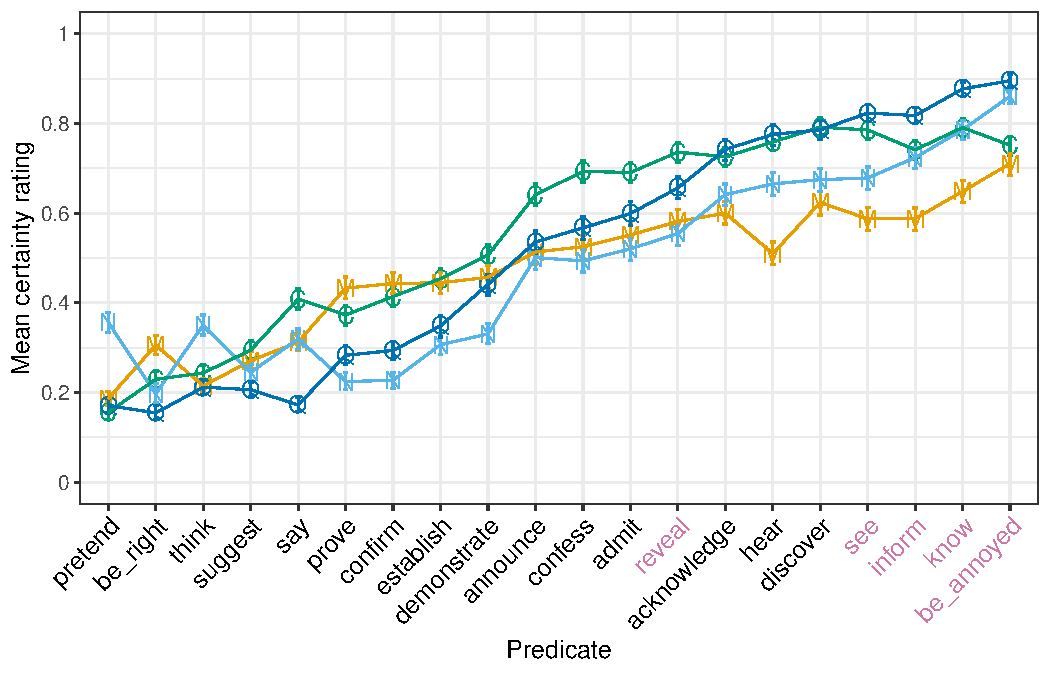
\includegraphics[width = \linewidth]{predicate-operator-graph-1}
				\caption{Mean certainty ratings by predicate and operator with 95\% bootstrapped confidence intervals. Embedding operator coded by letter and color:  \texttt{N} (light blue): negation, \texttt{M} (orange): modals, \texttt{C} (green): conditional antecedents, \texttt{Q} (dark blue): polar questions.}
				\label{fig:op-pred-ratings}
			\end{figure}

			Our results therefore provide further support from negation, modals, and conditionals for the result of \citet{degen_are_2022}, that projection does not categorically differentiate between (semi-)factive and non-factive predicates, while also replicating it for polar questions. The CCs of non-factive \emph{inform} and \emph{acknowledge}, for instance, are at least as projective as that of some (semi-)factive predicates.

		\subsubsection{By-predicate variation in the effect of operator}

			We observe differences between predicates in by-operator variation, i.e., a operator/predicate interaction effect, which is also illustrated in Figure~\ref{fig:op-pred-ratings}.
			%
			For instance, whereas the CC of \emph{be annoyed} projects more from under negation and questions than conditionals and modals, and the CC of \emph{discover} projects less from negation than conditionals and questions, and more from under negation than modals. The CC of \emph{know} projects less from under negation than questions, but more from under negation than modals, while the difference between negation and conditionals is not significant.
			%
			These generalizations are supported by models\ \# 2--4 in Table\ \ref{t:models}, which also each have at least $34$ highly significant interaction terms (out of $57$ possible interactions of operator and predicate).

			\begin{table}[ht]
				\centering
				\begin{tabular}{llrrrr}
					Model & & Estimate & Std. Error & t-value\\
					\midrule
					\#2 & Intercept: \emph{\bf be annoyed}/negation & 0.87 & 0.01 & 79.86 & ***\\
					& operator: conditional & -0.12 & 0.02  & -7.36 & ***\\
					& operator: modal & -0.16 & 0.02  & -10.01 & ***\\
					& operator: question & 0.02 & 0.01 & 1.72 & n.s.\\
					\midrule
					\#3 & Intercept: \emph{\bf discover}/negation & 0.68 & 0.01 & 62.70 & ***\\
					& operator: conditional & 0.11 & 0.02 & 7.11 & ***\\
					& operator: modal & -0.06 & 0.02 & -3.63 & ***\\
					& operator: question & 0.10 & 0.01 & 7.08 & ***\\
					\midrule
					\#4 & Intercept: \emph{\bf know}/negation & 0.79 & 0.01 & 72.97 & ***\\
					& operator: conditional & 0.00 & 0.02 & -0.06 & n.s.\\
					& operator: modal & -0.14 & 0.02 & -9.18 & ***\\
					& operator: question & 0.08 & 0.01 & 5.67 & ***\\
					\bottomrule
				\end{tabular}
				\caption{\small Excerpt of the output from three linear mixed effects models, with fixed effects: operator, predicate, and their interaction; random effect: participant intercepts.
				Models were fit with \texttt{lme4, lmertest} in \texttt{R}. Models \textbf{\#2--4} also had at least $34$ highly significant interaction terms of \texttt{operator} and \texttt{predicate} with $p < 0.001$ (not shown here).\label{t:models}}
			\end{table}

			Our result that by-operator projection variability interacts with predicate concurs with \citet{smith_relationship_2014}, while we did not reproduce their result that the CC of \emph{know} projects more from negation than conditionals (we found no difference here). Our results differ from those of \citet{sieker_projective_2022}, who found no difference between the two groups of predicates they assumed in the effect of operator.
			%
			However in line with Sieker \& Solstad, our results question \posscite{karttunen_observations_1971} proposed difference between factive and semi-factive predicates (see also \citealt{beaver_have_2010}). Although our data replicate the result from \citet{tonhauser_how_2018} that, in polar questions, the CC of semi-factive \emph{discover} is less projective than that of \emph{know}, the same does not hold in conditionals, contrary to what would be expected based on \posscite{karttunen_observations_1971} distinction between factive and semi-factive predicates.
			%
			Further, the CC of (factive) \emph{be annoyed} does not project invariably from all four operators, and the CC of \emph{discover,}  which is considered semi-factive, does not project more from under negation than the other three operators. The pattern observed for {\em know} does not fit into either category.

		\subsubsection{Converging evidence for operator / predicate interactions}

			Our experimental result that that the effect of entailment-cancelling operator differs by predicate finds further support in the data from \posscite{white_role_2018} MegaVeridicality dataset.
			%
			White \& Rawlins assess projection inferences associated with 517 clause-embedding predicates by presenting them in 50 \lq low-content\rq\ syntactic frames, like the ones in \Next, illustrated here with \textit{know}. The frames in \Next present predicates associated with projective contents embedded under negation \Next[a], in conditional antecedents \Next[b], or both \Next[c], in combination with a projection question (\textit{Did that thing happen?}).

			\ex. \a. Somebody didn’t know that a particular thing happened. Did that thing happen?
				\b. If somebody knows that a particular thing happened, did that thing happen?
				\b. If somebody didn’t know that a particular thing happened, did that thing happen?
				\z.
			\z.

			In a series of experiments, participants presented with stimuli like \Last responded with \lq yes\rq, \lq no\rq, or  \lq maybe\rq (coded as \texttt{1, -1,} or \texttt{0}, respectively). Here, we present data from their data set, for the frames in \Last, and 16 of their predicates. These include ones also used in our experiment as purported factives (\textit{be annoyed, know, reveal}) and semi-factives (\textit{discover, see}), and eleven further predicates commonly characterized as factive or semi-factive (\textit{amuse, find out, forget, learn, love, notice, realize, recognize, regret, remember, understand}).

			The mean projection ratings by embedding context and predicate are presented in Figure~\ref{fig:figure4}, which shows that effect of embedding context on projection differs by predicate.

			For instance,\footnote{Give some examples of differences here, but first double check if lines are labeled correctly. Also angle labels on x-axis.}

			% the predicates \textit{see} and \textit{learn} have the same mean ratings for both negative and conditional contexts. However, the effect of negative conditional contexts does not simply reflect the additive result of both effects, but 

			\begin{figure}[ht]
				\centering
				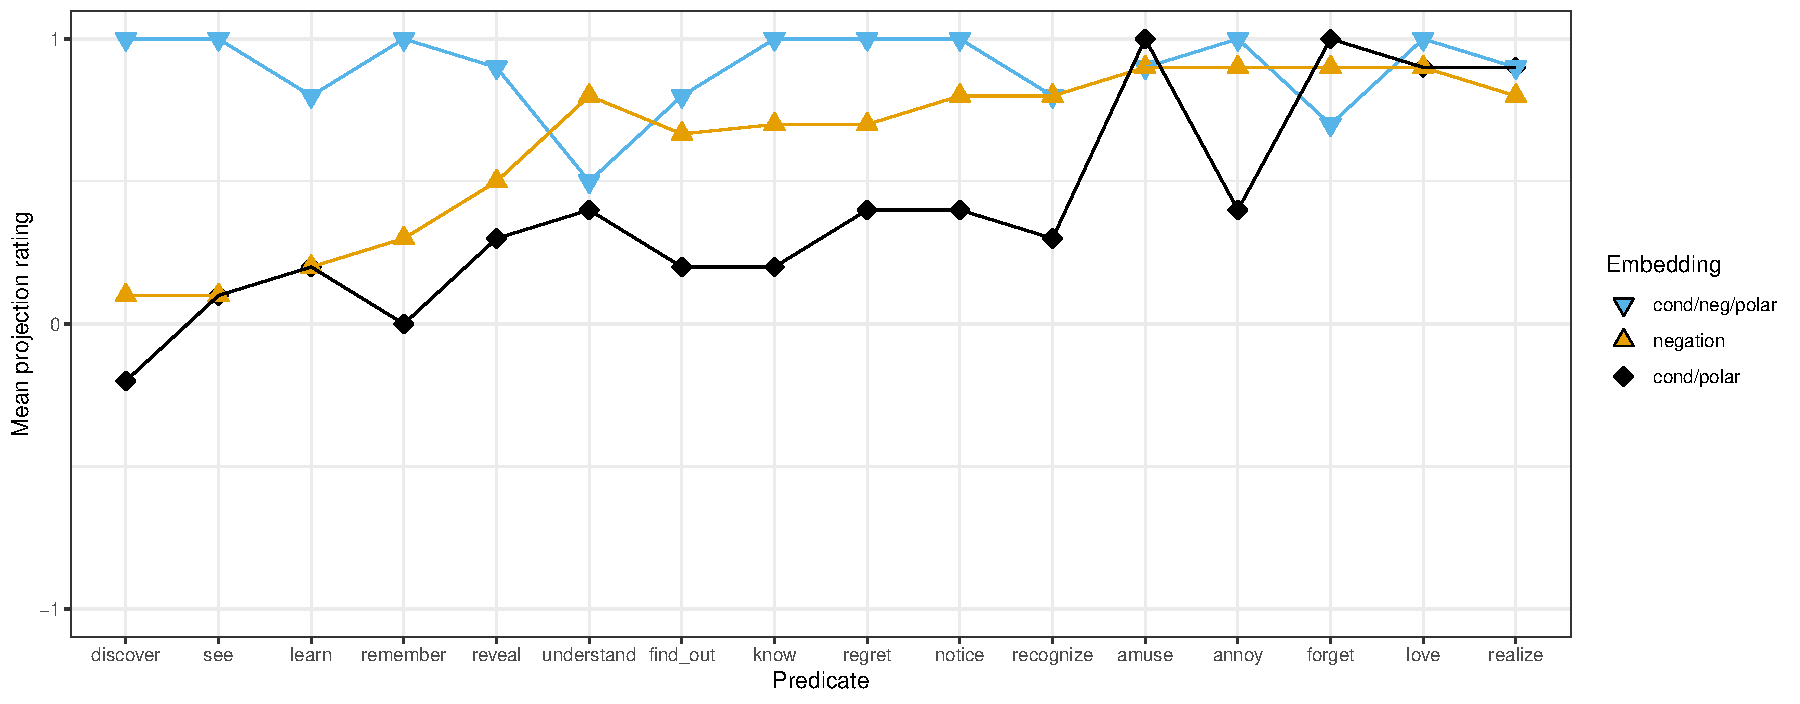
\includegraphics[width = \linewidth]{mega-veridicality}
				\caption{Mean projection ratings by embedding context and predicate.}
				\label{fig:figure4}
			\end{figure}

			It is worth noting that the task assesses global projection only in case of \Last[a], but not \Last[b+c], where the question \textit{did it happen?} is embedded in the conditional consequent. It assesses whether the projective inference holds in the conditional local context. Nevertheless, the data provides supporting evidence for by-predicate variation in the effect of operators on projection. Crucially, the by-predicate variation in the effect of negation in the global context is different from the by-predicate variation in the effect of negation in the conditional context.


		\subsubsection{Interim conclusion}

			Based on our data, we conclude that embedded propositional content projects differently from under different entailment-cancelling operators. A methodological implication of this finding is that claims about projection variability must be relativized to the entailment-canceling operator in future research.
			%
			Further, the observed by-predicate variation does not categorically distinguish between lexical classes (e.g., factives, semi-factives, veridical predicates), so future research appealing to these categories must clarify their definition.
			%
			Finally, the effect of operator on projection differs by predicate. The theoretical implications of our findings are discussed in the following section. Importantly, accounts of projective content need to take into account predicate/operator interactions, and the gradient by-predicate variability.


\section{Theoretical implications}
	Our results---that projection is modulated by entailment-canceling operators, that there is by-predicate variation in the effect of operator on projection, and that this variation is gradient in ways that cannot be predicted by categorical lexical classes---are not captured by contemporary projection analyses.
		
		Here, we discuss this for (i) dynamic approaches, which assume that projection is determined lexically for factive predicates (\citealt{heim_projection_1983,heim_presupposition_1992,van_der_sandt_presupposition_1992}), (ii) approaches which assume that projection is determined by a triggering algorithm based on information structure that operates over the literal entailments of an utterance (\citealt{abrusan_predicting_2011,simons_best_2017}), and (iii) approaches with a triggering algorithm based on world-knowledge that operates over contextual entailments of an utterance (\citealt{schlenker_triggering_2021}). While all of these approaches meet limitations in accounting for our data, we argue that the observed gradient effects of predicate/operator interactions favor integrating insights from competing accounts, namely a contextual triggering algorithm (as in \citealt{abrusan_predicting_2011,simons_best_2017}) operating over contextual set of inferences (as in \citealt{schlenker_triggering_2021}).
	
	\subsection{Lexical triggering in dynamic semantics}

		Dynamic semantic accounts of projection (e.g., \citealt{heim_projection_1983,heim_presupposition_1992,van_der_sandt_presupposition_1992}) assume lexical triggering: there is a class of (semi-)factive predicates, which lexically presuppose their CCs. Presupposed CCs project to the global context, except when that would produce an inconsistency, in which case they are accommodated to the local context of the operator.

		\paragraph{By-operator variation.} In our study, the stimulus utterances were presented out of the blue, leaving it to the participants to imagine a suitable discourse context. Therefore, none of the CCs should be interpreted as necessarily inconsistent with contextual information.
		%
		Consequently, dynamic approaches do not lead us to expect differential effects of entailment-cancelling operators on projection in out-of-the blue contexts. Instead, negation and conditional antecedents are given a semantics that derives their behavior as presuppositional \lq holes\rq\ (in the sense of \citealt{karttunen_observations_1971}). For instance in \citealt{heim_projection_1983}, presuppositional expressions in negative prejacents and conditional antecedents are evaluated relative to the global context set. Therefore, presuppositional expressions in these contexts are predicted to behave like unembedded ones, with no expected differences. While the approach does not explicitly address epistemic possibility modals or polar questions, we might expect that they would be treated as presuppositional holes along the same lines.
		%
		Differential effects of operators on projection could conceivably be addressed in such a system by assuming that the meaning of entailment-cancelling operators systematically affects the possibility of local accommodation (e.g., by assuming that accommodation is more likely under modals than conditional antecedents). However, no such effects have been spelled out.
		
		\paragraph{Gradient by-predicate variation.} The assumption of categorical lexical triggering does not address the projection variation among purported factive predicates (see also discussion in \citealt{degen_are_2022}). It also cannot address the fact that the CCs of some non-factive predicates (e.g., \emph{inform, acknowledge}) project just as much, or more, than some (semi-)factive predicates (e.g., \emph{reveal, discover, see}). That is because, it only makes predictions for the projection of the CC of (semi-)factive predicates, whose CCs are analyzed as presuppositions. It therefore does not address the data for the non-veridical predicates in our study.
		%
		Further, the categorical lexical distinctions are not sufficiently fine-grained to make predictions about the gradient by-predicate variation in the effect of operator on projection.
		%
		This interaction effect can only be addressed by taking into account more fine-grained lexical distinctions than assuming that some predicates are presuppositional, while others are not.


	\subsection{Triggering based on information structure} % (fold)
		The information-structural triggering approaches in \citealt{abrusan_predicting_2011} and \citealt{simons_best_2017} assume that projection is not determined lexically, but by a triggering mechanism, which operates over the entailments of an expression, and determines which of them projects. They assume entailments project that do not contribute to the main point invoked by the utterance.

		% Instead of assuming that the possibility of projection is determined lexically, the accounts in \cite{abrusan_predicting_2011,simons_best_2017} and \citet{schlenker_triggering_2021} assume a triggering mechanism, which operates over a set of inferences associated with an utterance, and determines which of them projects. The assumed triggering mechanisms differ on two dimensions: (i) how the set of inferences is determined that constitutes the input to the triggering mechanism, and (ii) the algorithm by which these inferences are derived as projective or not.

		For instance, \citet{simons_best_2017} operationalize the main point of an utterance in terms of at-issueness relative to the Question Under Discussion (QUD, see \citealt{roberts_information_1996,roberts_information_2012}). 
		%
		In the QUD-based approach to information-structure in discourse, each utterance addresses a question, which is determined by its alternative-structure, which, can be indicated by focus-marking. For example, in a modalized utterance with \emph{be annoyed}, the CC can be focused \Next[b], which leads to the alternative structure in \Next[c], allowing the utterance to address a question like \Next[a].

		\ex. \a. What was Cole annoyed about today?
			\b. Perhaps Cole was annoyed [$_F$ that Julian dances salsa].
			\b. $\{p \mid \exists q(p = \lambda w.$\emph{Cole was annoyed that} $q$ \emph{in} $w)\}$
			\z.
		\z.

		In contrast, focus on the subject \Next[b] leads to the alternative structure in \Next[c], allowing the utterance to address a question like \Next[a].

		\ex. \a. Who was annoyed today?
			\b. Perhaps [$_F$ Cole] was annoyed that Julian dances salsa.
			\b. $\{p \mid \exists x(p = \lambda w.x$ \emph{was annoyed in} $w$ \emph{that Julian dances salsa}$)\}$
			\z.
		\z.

		The account assumes that an inference projects if it is entailed by the union of the alternatives (see also \citealt{abusch_presupposition_2010}). therefore predicting projection of the CC in \Last, but not \LLast. That is, under the assumption that $x$ \emph{was annoyed that} $p$ entails $p$.

		\paragraph{Gradient by-predicate variation.} The triggering mechanisms assumed in \citealt{abrusan_predicting_2011} and \citealt{simons_best_2017}, predict a potential of projection for inferences that are entailed by the literal content of the modal prejacent $p$ in \Last and \LLast, and similarly for propositions embedded in negative contexts, conditional antecedents and polar questions. These accounts, therefore, predict a potential of projection for CCs that are entailed by the prejacent, due to the lexical entailments of veridical predicates, or due to entailments that are contributed compositionally by the literal content (see e.g., \citealt{roberts_i_2019}). However, they do not make systematic predictions for CCs, such as in \Last, that are not entailed. As a result, these accounts cannot address the fact that we see some amount of projection for all of the tested predicates.

		Because the main point of an utterance is often determined in the discourse context (\citealt{roberts_information_1996,roberts_information_2012}, \emph{et seq.}), these approaches incorporate discourse effects on projection.
		%
		% \citet{abrusan_predicting_2011} also makes predictions for utterances in out-of-the-blue contexts: Utterances are associated with a default main point that is grammatically determined by the time at which the matrix predicate is interpreted.
		%
		The account in \citealt{simons_best_2017} could be extended to address our gradient data in out-of-the blue contexts, by assuming (i) that embedded contents that are not at-issue can project even if they are not entailed, and (ii) that linguistic expressions differ in how likely the contributed contents are interpreted as at-issue (as suggested in \citealt{tonhauser_how_2018}).
		%
		In our data, for instance, the CC of \emph{discover} \Next[a] has received relatively high projection ratings, while that of \emph{confirm} \Next[b] has received medium to low ratings. To explain this difference, the information-structure based triggering approach would need to assume that the CC of \emph{discover} is less likely to be at issue than that of \emph{confirm}.

		\ex. \a. Perhaps Cole discovered that Julian dances salsa.
			\b. Perhaps Cole confirmed that Julian dances salsa.
			\z.
		\z.

		While \citet{tonhauser_how_2018} experimental evidence that projection ratings negatively correlate with at-issueness ratings in out-of-the-blue polar questions. \citet{sieker_projective_2022} argue that their data also shows the same correlation for modal, conditional antecedent, and negation contexts for the German clause-embedding predicates they investigated. To address the gradient by-predicate variation theoretically, this approach would need to explicitly spell out how various predicates are associated with different likelihoods that their CCs is interpreted as at-issue.

		\paragraph{Operator/predicate interaction.}
			Since we found an operator/predicate interaction effect on projection, a further prediction of this type of approach would be that at-issueness ratings would show an operator-predicate interaction in this experimental setup as well. To address the interaction effect theoretically, an information structural triggering approach would need to make explicit predictions about how the meaning of entailment-cancelling operators affects at-issueness differentially for different predicates. This is certainly conceivable, when we take default assumptions about how likely embedded contents are interpreted at issue to be associated with the entire embedding context, including clause-embedding predicates, but also entailment-cancelling operators. However, this has not been spelled out explicitly and needs to be investigated in more detail.
			

	\subsection{Triggering based on world knowledge}

			The account in \citealt{schlenker_triggering_2021} assumes a triggering mechanism which operates on local contextual entailments of an expression, and determines which one of them projects based on probabilistic world knowledge about the truth of the invoked contents. For instance, in a negated utterance with \emph{discover} \Next[a], the CC expressed by \Next[c] has the potential to project if it is entailed by the negative prejacent \Next[b] along with the information that is available in its local context. Based on \citealt{heim_projection_1983} and \citealt{schlenker_local_2009}, negation is treated as a presuppositional hole, and the local context under negation is taken to be the global context.

			\ex. \a. Cole didn't discover that Julian dances salsa.
				\b. Cole discovered that Julian dances salsa.
				\b. Julian dances salsa.
			\z.

			The triggering mechanism states that an inference $p$ of some propositional expression $E$ projects if $p$ is an epistemic precondition for the truth of $E$ in its local context $c^\prime$.
			%
			$p$ is an epistemic precondition of $E$ in $c^\prime$ if, usually, when one acquires the belief in $c^\prime$ that $E$, one already knows that $p$.
			%
			For \Last[a], the CC expressed by \Last[c] can be characterizes as an epistemic precondition for the negative prejacent \Last[b] based on the \lq subjective conditional probability\rq\ that a generic epistemic agent would already believe \Last[c] when learning that \Last[a] is true given the local context. Specifically, it is taken to be an epistemic precondition, if that probability reaches a contextually given threshold.

			\paragraph{Gradient by-predicate variation.} This account predicts the potential of projection for CCs that are entailed by the prejacent in combination with contextual information. It can therefore incorporate effects of contextual information on projection, such as the reliability of the source of a speech report (\citealt{rieh_credibility_2010,de_marneffe_did_2012}). It also predicts the potential to of projection for CCs that are not entailed based on the literal content. In order to extend an account along these lines to address the out-of-the-blue utterances in our study, we might assume that these out-of-the-blue utterances are interpreted relative to an imagined plausible discourse context (c.f., discussion in \citealt{simons_best_2017}).

			Due to the probabilistic nature and context-sensitivity of the triggering mechanism, the approach can make gradient predictions. However, the subjective conditional probabilities associated with expressions and their contextual inferences are taken as given in the account. In order to make concrete predictions about the gradient by-predicate variation, this account would need to make explicit how the relevant probabilities are derived based on different predicates. For instance, to explain the contrast that \emph{discover} receives higher projection ratings than \emph{confirm}, this account would assume that the situations in which one learns that a sentence like \emph{$x$ discovered that $p$} is true, are such that one already knew that $p$ is true more often than situations in which one learns the truth of a sentence like \emph{$x$ confirmed that $p$}.

			\paragraph{By-operator variation.} The account does not incorporate differential effects of entailment-cancelling operators on projection. Although subjective conditional probabilities are relativized to a local context, the local context in negative contexts and conditional antecedents is assumed to the global context (based on \citealt{heim_projection_1983,schlenker_local_2009}). Therefore, no differential effect of operator is expected. For instance, the conditional probability for $p$ given $E$ vs that of $p$ given $(\emph{not } E)$ or that of $p$ given $(\emph{if } p, q)$ should not differ.

			In order to address the operator-predicate interaction effect, an approach based on epistemic preconditions would need to make explicit how the meaning of entailment-cancelling operators affects the conditional probabilities differentially for different predicates.
			%
			The conditional probability that some embedded content is antecedently known would need to be computed relative to a global context, and take into account the entire embedding context, including the combination of entailment-cancelling operator and clause embedding predicate.

	\subsection{Discussion: Contextual inferences and probabilistic triggering}

		Our data showed gradient projection variation, based on a main effect of predicate, and an operator-predicate interaction. We found these effects for the CCs of clause-embedding predicates under four entailment-cancelling operators in out-of-the-blue contexts. The fact that we see some amount of projection for all predicates (even non-veridical ones), can only be addressed by an account that assumes the potential of projection for contextual inferences, rather than only literal ones.

		The main effect of predicate and the operator-predicate interaction are both gradient effects, and cannot be explained by a categorical distinction between presuppositional and non-pre\-suppo\-si\-tion\-al predicates. The effects could rather be addressed in a probabilistic account, where various embedding contexts (i.e., combinations of entailment-cancelling operator and predicate) are associated with different probabilities that the embedded content projects.

		Under the assumption of information-structural triggering, this is the probability that the embedded content is not at issue in the (possibly imagined) discourse context. Under a world-knowledge-based triggering account, the projection probability can be associated with the probability that the embedded content is already known in the discourse context. These two notions are, of course, related. If some proposition is already known, raising an issue about whether $p$ is the case will be uninformative. Therefore, it is unclear whether these two approaches would make different predictions for our data. Both types of accounts would need to be extended to make concrete predictions for the contribution of the combinations of entailment-cancelling operators and predicates.

\section{Lexical differences}
	Can the observed interaction between predicate and operator in mean projection ratings be predicted from lexical semantic/pragmatic properties of the predicates, and, if so, how?
	This is a pressing question for future research, to which our data offer some tentative answers. We can find some initial generalizations over lexical properties, indicated in \textbf{Figure~\ref{fig:patterns}}, which gives the mean certainty ratings for the four operators by predicate, identifying four groups of predicates that show similar by-operator variation.
	
	\begin{figure}[ht]
		\centering
		% \hspace{-.5em}\resizebox{\linewidth}{!}{
		\begin{tabular}{p{.205\linewidth} p{.18\linewidth} p{.18\linewidth} p{.18\linewidth} p{.18\linewidth}}
			\footnotesize \hspace{2.1em} (a) Negation high &
			\footnotesize \ (b) Negation low &
			\footnotesize (c) Conditional high &
			\footnotesize \ (d) Modal low
			% & \footnotesize \  (e) Discover
			\\
			\vspace{-.6\baselineskip}
			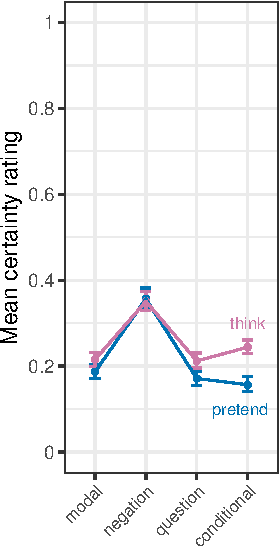
\includegraphics[width=.225 \textwidth, valign=T]{negation-high-1.pdf}
			&
			\vspace{-.6\baselineskip}
			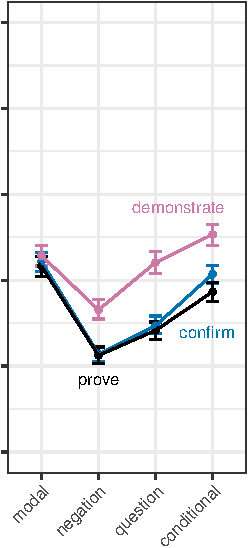
\includegraphics[width=.2\textwidth, valign=T]{negation-low-1.pdf}
			&
			\vspace{-.6\baselineskip}
			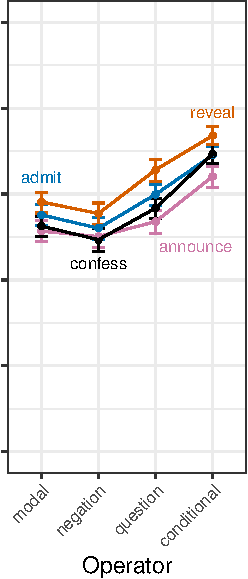
\includegraphics[width=.2\textwidth, valign=T]{conditional-high-1.pdf}
			&
			\vspace{-.6\baselineskip}
			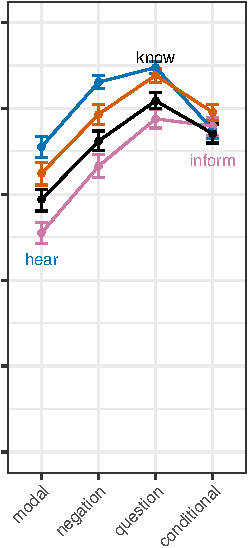
\includegraphics[width=.2\textwidth, valign=T]{modal-low-1.pdf}
			% &
			% \vspace{-.6\baselineskip}
			% 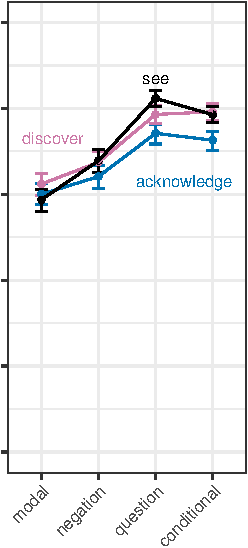
\includegraphics[width=.2\textwidth, valign=T]{discover-1.pdf}
			\\
		\end{tabular}
		% }
		
		\caption{Mean certainty ratings by operator with $95\%$ bootstrapped confidence intervals, for some groups of predicates (\lq predicate patterns\rq).}
		\label{fig:patterns}
	\end{figure}

	
	%
	The non-veridical predicates \emph{pretend} and \emph{think} exhibit the `Negation high' pattern, shown in panel (a) of Figure~\ref{fig:patterns}. These are the only predicates that are most projective under negation compared to all other operators. This could be related to 
	assumptions that non-veridical doxastics like \emph{think} can often be interpreted in comparison to a stronger veridical alternative (e.g., \citealt{heim_artikel_1991,chemla_epistemic_2008}). We tentatively hypothesize that this can lead to an inference that the CC is false in upward-monotone contexts, but not under negation. A similar alternative seems to be salient for \emph{pretend}, but not the non-veridical communicative predicates \emph{say} or \emph{suggest}.
	
	The inferential predicates \emph{confirm, demonstrate}, and \emph{prove} exhibit a `Negation low' pattern, shown in panel (b). These are most projective under modals and conditionals and least projective under negation. Here, we may hypothesize that a negative statement involving these predicates is often only taken as relevant (in a Gricean sense) when it is antecedently known that there was an attempt to confirm/demonstrate/prove the truth of the CC. This may result in an inference that this attempt failed and result in lower projection ratings under negation.
	
	For \emph{admit, announce, confess}, and \emph{reveal}, the CC is most projective when embedded in conditional antecedents: This `Conditional high' pattern (c) may suggest that the discourse effect of a conditional interacts with these change-of-state communication predicates.
	
	Finally, the predicates \emph{hear, inform,} and \emph{know} exhibit a `Modal low' pattern (d). The lexical meaning of these predicates, whose CCs are among the most projective, appears to interact with the modal adverb {\em perhaps}, yielding lower projection ratings.

\section{Conclusion}


% \newpage
\bibliographystyle{sub-chicago}
\bibliography{projection}

\end{document}
